\subsection{Repräsentativer Anwendungsfall für die Energiewirtschaft}\label{usecase}

Die verschiedenen Werttreiber und Anforderungen für ein Digitalisierungskonzept unterscheiden sich je nach Unternehmen und Branche.
Für eine erfolgreiche Transformation müssen daher individuelle Anwendungsfälle identifziert werden.
In Anbetracht der Dynamik und des rasanten Tempos, in der neue Technologien entstehen,
ermöglicht ein anwendungsfallbasierter Ansatz eine flexible und agile Anpassung. \citep[S. 31]{Acharya2019}
\\Aus diesen Gründen wird im Folgenden ein repräsentativer Anwendungsfall für die Energiebranche
und den damit entstehenden Anforderungen dargestellt.

\subsubsection{Ausgangssituation}

Der deutsche Windenergieanlagenhersteller Enercon GmbH aus Aurich ist mit über 29000 Anlagen in 45 Ländern ein Global Player in der Branche. Da das Kerngeschäft des Unternehmens auf dezentraler Energieproduktion basiert, hat Industrie-4.0-Fähigkeit einen besonderen Stellenwert. Sei es die Einspeisung der produzierten Energie in das Smart-Grid, die Fernsteuerung oder die Zustandsüberwachung der Anlagen und Windparks: Das unternehmenseigene \acf{scada}-System ist auf die Enercon-Anlagen abgestimmt bietet umfangreiche Lösungen für die Kunden. Als Kunden stehen die Energieversorgungsunternehmen im Vordergrund, welche sowohl auf Anforderungen der Netzbetreiber als auch der eigenen Kunden, also der Konsumenten, reagieren müssen. Im Kontext des Unbundlings des Energiemarktes etablierte sich die Branchenlösung \acf{sapisu}, welches Bestandteil von SAP ERP ist, als Vertriebs- und Informationssystem für \ac{evu}. Auch die Enercon-IT nutzt SAP-Produkte für das Management der Ressourcen, Logistik oder Kunden. Im Zuge der Anpassung an die Anforderungen der digitalen Welt wird SAP jedoch den Support der bisher auch von Enercon verwendeten Standard-ERP-Software bis 2025 einstellen. Der Fokus wird auf das Nachfolgeprodukt SAP S/4 HANA gesetzt, welche die echtzeitfähige In-Memory-Datenbanktechnologie \acf{hana} für nutzt. Aus dem Grund bereitet sich Enercon rechtzeitig auf die Migration auf S/4 HANA vor. Die Integrations- und Entwicklungsplattform von \ac{hana} bietet zahlreiche Möglichkeiten zur Realisierung von innovativen Softwarelösungen sowohl auf der Cloud als auch On-Premise. Die Neuausrichtung der IT-Architektur ist auch für die erfolgreiche digitale Transformation von Enercon großer Bedeutung.

\noindent Im besonderen Interesse liegt die SAP Leonardo \ac{iot} Foundation, vor allem in Anbetracht einer möglichen Integration von Stammdaten aus dem S/4 HANA System. Dafür ist zunächst eine Analyse der SAP Leonardo Systemarchitektur mitsamt der Perspektiven gewünscht. Dies könne als Entscheidungsgrundlage für eine Erweiterung des Geschäftsfeldes von Energieproduktion auf IT-Dienstleistungen dienen. Außerdem soll prototypisch dargestellt werden, inwiefern sich SAP Leonardo IoT als Verwaltungsschale für die Industrie-4.0-Komponente eignet. Langfristiges Ziel des Unternehmens sei es, das \ac{scada}-System über die Kommunikationsschnittstelle mit dem OPC XML-DA Protokoll echtzeitfähig zu gestalten. Um Risiken vor Inbetriebnahme und Kosten zu minimieren soll jedoch zunächst eine einfache Simulation genügen.

\noindent Die Simulation soll dem Servicepersonal in der Wartung ermöglichen, die Zustandsdaten des digitalen Zwillings einer Anlage in Echtzeit zu überwachen. Wenn kritische Messwerte empfangen werden, soll das Personal sofort benachrichtigt werden, damit Wartungsmaßnahmen eingeleitet werden können. Die Softwareentwickler/innen sollen den Prototypen beliebig sowohl um (Mess-)Geräte als auch um App-Funktionalitäten erweitern können.

\subsubsection{Anforderungserhebung}

Um die Anforderungen für die Umsetzung einer repräsentativen Lösung zu ermitteln, muss zunächst ermittelt werden, welche Einflussfaktoren sich im Kontext des Zielsystems befinden und wo sich die Grenze des Systems befindet. Diese Herangehensweise dient dazu, Probleme, Anforderungen und Lösungen für verschiedene Abstraktionsebenen zu definieren. Nach dem PAL-Modell kann auf die Kontext-, System- sowie die auf technische Ebene abstrahiert werden \citep{Lauenroth2016}.

\begin{figure}[h]
  \centering
  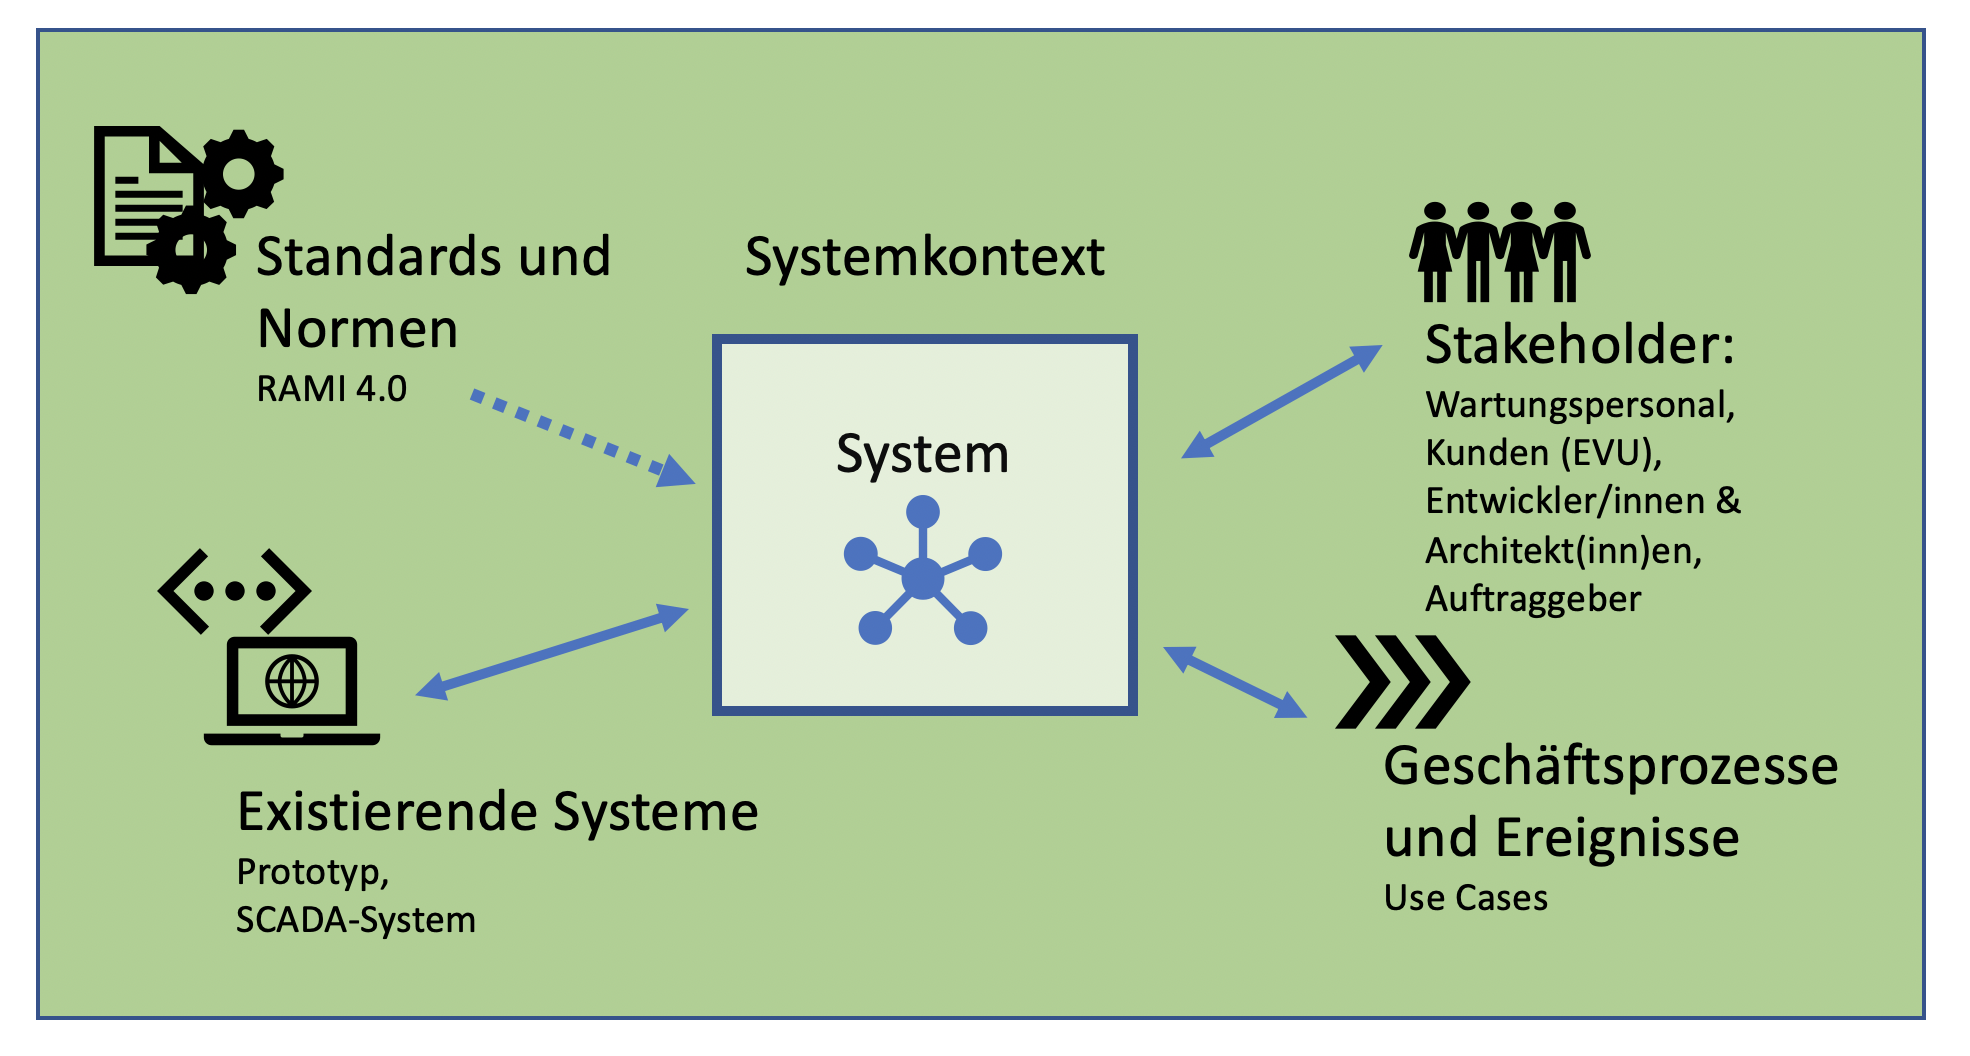
\includegraphics[width=1\linewidth]{System_Kontext.png}
  \caption[Das System und der Systemkontext]{Das System und der Systemkontext}
  \label{}
\end{figure}

\begin{itemize}
  \item Systemgrenzen und Systemkontext identifizieren
  \item Anforderungsquellen
  \item  \begin{itemize}
    \item RAMI 4.0
    \item Prototyp kann auch als Anforderungsquelle dienen
    \item Stakeholder ermitteln: Wer hat direkten/indirekten Einfluss auf Anforderungen z.B.  Nutzer des Systems oder Auftragsteller in Organisation
    \item Dokumente mit Einfluss z.B. Normen oder Standards, die in Referenzen wie RAMI vorhanden sind -> z.B. die Verwaltungsschale erklären und die expliziten Anforderungen im nächsten Subkapitel
    \item Existierende Systeme: Systeme, die mit dem geplanten System interagieren sollen oder Systeme, die auf ähnliche Weise bereits Existierende
    \item Beobachtbare Ereignisse oder Prozesse
    \item irrelevante Umgebung
  \end{itemize}
  \item Trennung von Problem , Anforderung und Lösung
\end{itemize}



Anforderungsquellen: RAMI 4.0 hinsichtlich Info-Layer



\subsubsection{Anforderungen}


\begin{table}[h]
  \begin{tabular}{ |p{5cm}|p{5cm}|p{5cm}| }
    \toprule
    Problem & Anforderung & Lösung \\
    \midrule
    \multicolumn{3}{ |l| }{\textbf{Kontextebene} }\\
    \hline
    K-P-1: Blacffdfdfjhdjfhfdhdfjhdfjhdfjhdfjhfdfdhdfjh & K-QA-1: Bkaffdddfsfdfssffsdfsddfsffsd  & K-L-1: Bremsen hhfdsdfsssssssdfdsfsdfdh\\
    \hline
     \multicolumn{3}{ |l| }{\textbf{Systemebene} }\\
     \hline
     S-P-1: Blacffdfdfjhdjfhfdhdfjhdfjhdfjhdfjhfdfdhdfjh & S-QA-1: Bkaffdddfsfdfssffsdfsddfsffsd  & S-L-1: Bremsen hhfdsdfsssssssdfdsfsdfdh\\
  \hline
    \multicolumn{3}{ |l| }{\textbf{Technische Ebene} }\\
    \hline
    T-P-1: Blacffdfdfjhdjfhfdhdfjhdfjhdfjhdfjhfdfdhdfjh & T-QA-1: Bkaffdddfsfdfssffsdfsddfsffsd \newline T-FA-1: Funktionale Anf & T-L-1: Bremsen hhfdsdfsssssssdfdsfsdfdh\\
    \bottomrule
    \end{tabular}
    \label{pal_table}
  \caption{PAL-Tabelle}
\end{table}



Was muss das System können? An RAMI orientieren -> Was muss erfüllt werden ?
Scada macht über Protokolle und Schnittstellen Telemetriedaten der Windenergieanlage
schreibt das Lokal in eine DB und erzeugt Alarmmeldungen
quittieren lokal am Rechner
alle 10 Minuten --> mit Leonardo schnellere Reaktion in Echtzeit
50 Hz Frequenz -> muss gehalten werden, um schnell auf Probleme reagieren zu können


\begin{itemize}
  \item erneuerbare Energien werden von der Plattform Industrie 4.0 kaum berücksichtigt !
  \item Was Kann SCADA-System? daten erfassen, an cloud senden, verarbeiten, digitaler zwilling unf steuern, aktionen und regeln für predictive Maintenance
  \item Fähigkeit, große Datenmengen auch offline zu verarbeiten -> Latenzprobleme
  \item ANFORDERUNG! WENN DIE Anlagen ins Smart Grid aufgenommen werden sollen, müssen sie Kommunikationsfähig sein!!!!
  \item Aus Requirements Engineering S. 10: Simulation vor Inbetriebnahme, um Fehler in Anforderungsanalyse festzustellen, damit Change Requests gemacht werden können
  \item Bei Anlagen, die mehrere Millionen Euro kosten, sind anders als in Software Mechanik und Elektronik eingebaut. Ein Change Request wäre viel zu teuer
  \item Anforderungsanalyse der Simulation beseitigt die Risiken nicht vollständig, da die Simulation nur so gut ist, wie man sich vorher Gedanken gemacht hat
  \item Welche Anforderungen ergeben sich aus dem Wandel?
  \item Anforderungen wie predictive Maintenance und Bezug auf RAMI 4.0.
  \item SAP als Tool, da Energiesektor hauptsächlich \acf{sapisu}
  \item Industrie 4.0-Komponente (Bitkom s. 52) mit verschiedenen Ebenene
\end{itemize}

\textbf{Anforderungen an Versorgungsunternehmen im Energiesystem der Zukunft \citep[S. 19]{Doleski2016}}

\paragraph{Merkmale von Akteuren in der digitalen Welt}
\begin{itemize}
  \item Allgegenwärtige Informationsverfügbarkeit
  \item Soziale Visualisierung1
  \item Absolute Mobilität
  \item Permanente Erreichbarkeit
  \item Lokalisierung
  \item Leistungsfähige Technologien
\end{itemize}

\paragraph{Wesentliche Herausforderungen für Energieunternehmen \citep[S. 21]{Doleski2016}}
\begin{enumerate}
  \item \textbf{Informationsflut}: zunehmendes Informationsangebot kann nicht oder nur bedingt aufgenommen werden
  \item \textbf{Informationsverarbeitung}: zunehmendes Informationsangebot kann nicht zu Wissen verarbeitet werden
  \item \textbf{Informationssysteme}: bestehende Informationssysteme liefern oftmals keine relevanten Informationen für die Unternehmensführung
\end{enumerate}
%


\paragraph{Einige Anforderungen an Versorgungsunternehmen}
Die Anforderungen sollen sich nur auf die Befähiger/Enabler sowie die Prozesse der Energieunternehmen beziehen
\begin{enumerate}
  \item Im Wettbewerb um geeignete Fachkräfte und Digital Natives bestehen $[Enabler]$
  \item Aufbau eines leistungsfähigen Informationsmanagements zur Speicherung, Verarbeitung und Auswertung sehr großer Datenmengen in Echtzeit $[Enabler]$
  \item Big Data beherrschen und innovative technische Lösungen anbieten $[Enabler]$
  \item Image eines verantwortungsbewusst handelnden Unternehmens schaffen und glaubhaft leben $[Enabler]$
  \item Kosteneffizient und professionell handeln $[Prozesse]$
  \item Veränderung von Organisation und Betriebsprozessen zügig vorantreiben $[Prozesse]$
  \item Alle Abläufe müssen modernen Datensicherheitsanforderungen entsprechen $[Prozesse]$
  \item uvm
\end{enumerate}
